\documentclass[11pt,a4paper]{article}
\usepackage{fontspec,geometry,graphicx,float,listings,tikz,hyperref}
\usetikzlibrary{positioning,arrows.meta}
\geometry{margin=1.8cm}\setmainfont{DejaVu Serif}
\lstset{language=Java,basicstyle=\ttfamily\scriptsize,breaklines=true,frame=single,columns=fullflexible}
\title{Devoir n°1 : Patrons de construction (INF461)}
\author{AMAYEN BOUSSIOM THIERRY MARTIN\\Matricule : 25I2177}\date{}
\newcommand{\boxe}[1]{\node[draw,rectangle,align=center,minimum width=3.2cm,minimum height=.85cm]{#1};}
\begin{document}\maketitle
\section*{Introduction}
Ce devoir présente deux exemples personnels des patrons Factory Method et Factory. Chaque exemple comporte d'abord trois classes concrètes, puis une version modifiée avec une quatrième classe. Les diagrammes montrent les relations entre le client, les fabriques et les objets créés.

\section{Factory Method : commandes de restaurant}
Une application de restauration crée une commande à partir du choix du client. La fabrique unique connaît les types de commandes.
\subsection{Exemple initial : trois commandes}
\begin{center}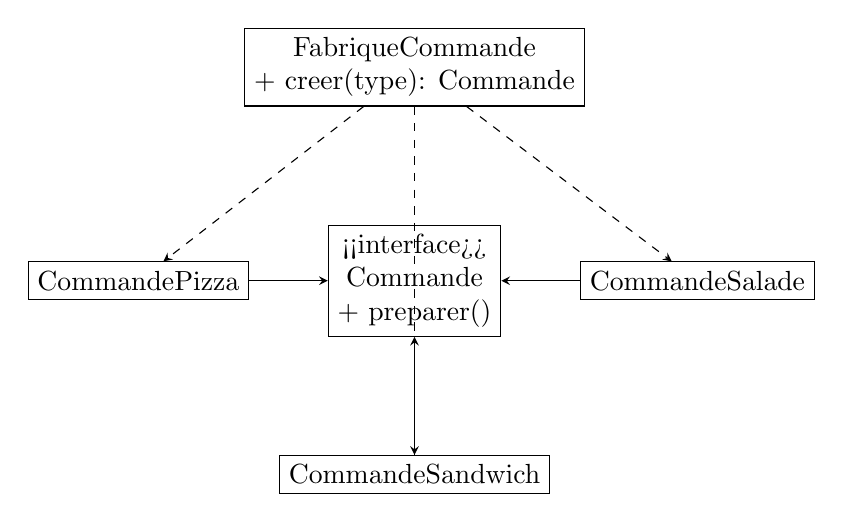
\begin{tikzpicture}[node distance=1.5cm and 1cm,>=stealth]
\node[draw,align=center] (f) {FabriqueCommande\\+ creer(type): Commande};
\node[draw,align=center,below=of f] (c) {<<interface>>\\Commande\\+ preparer()};
\node[draw,align=center,left=of c] (a) {CommandePizza};\node[draw,align=center,below=of c] (b) {CommandeSandwich};\node[draw,align=center,right=of c] (d) {CommandeSalade};
\draw[->,dashed] (f)--(a);\draw[->,dashed](f)--(b);\draw[->,dashed](f)--(d);\draw[->] (a)--(c);\draw[->](b)--(c);\draw[->](d)--(c);
\end{tikzpicture}\end{center}
\subsection{Variante : quatre commandes}
La classe \texttt{CommandeDessert} est ajoutée. \texttt{FabriqueCommande} reçoit aussi le type \texttt{dessert} ; la fabrique doit donc être modifiée.
\begin{center}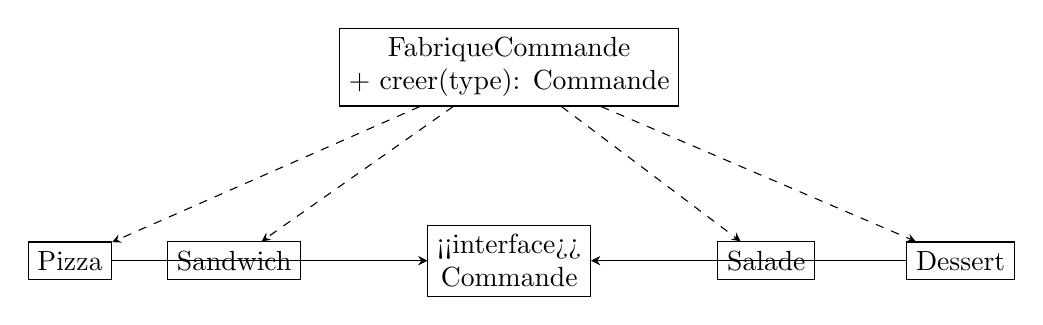
\begin{tikzpicture}[node distance=1.5cm and .8cm,>=stealth]
\node[draw,align=center] (f) {FabriqueCommande\\+ creer(type): Commande};\node[draw,align=center,below=of f] (c) {<<interface>>\\Commande};
\node[draw,align=center,left=4.0cm of c] (a) {Pizza};\node[draw,align=center,left=1.6cm of c] (b) {Sandwich};\node[draw,align=center,right=1.6cm of c] (d) {Salade};\node[draw,align=center,right=4.0cm of c] (e) {Dessert};
\draw[->,dashed](f)--(a);\draw[->,dashed](f)--(b);\draw[->,dashed](f)--(d);\draw[->,dashed](f)--(e);\foreach \x in {a,b,d,e}{\draw[->](\x)--(c);}
\end{tikzpicture}\end{center}
\begin{lstlisting}
interface Commande { String preparer(); }
class CommandePizza implements Commande { public String preparer(){ return "Pizza"; } }
class CommandeSandwich implements Commande { public String preparer(){ return "Sandwich"; } }
class CommandeSalade implements Commande { public String preparer(){ return "Salade"; } }
class CommandeDessert implements Commande { public String preparer(){ return "Dessert"; } }
class FabriqueCommande { Commande creer(String t) { return switch(t) {
 case "pizza" -> new CommandePizza(); case "sandwich" -> new CommandeSandwich();
 case "salade" -> new CommandeSalade(); case "dessert" -> new CommandeDessert(); default -> throw new IllegalArgumentException(); }; } }
\end{lstlisting}

\section{Factory : moyens de paiement}
Une application de vente utilise une fabrique abstraite. Chaque sous-classe crée son propre moyen de paiement.
\subsection{Exemple initial : trois paiements}
\begin{center}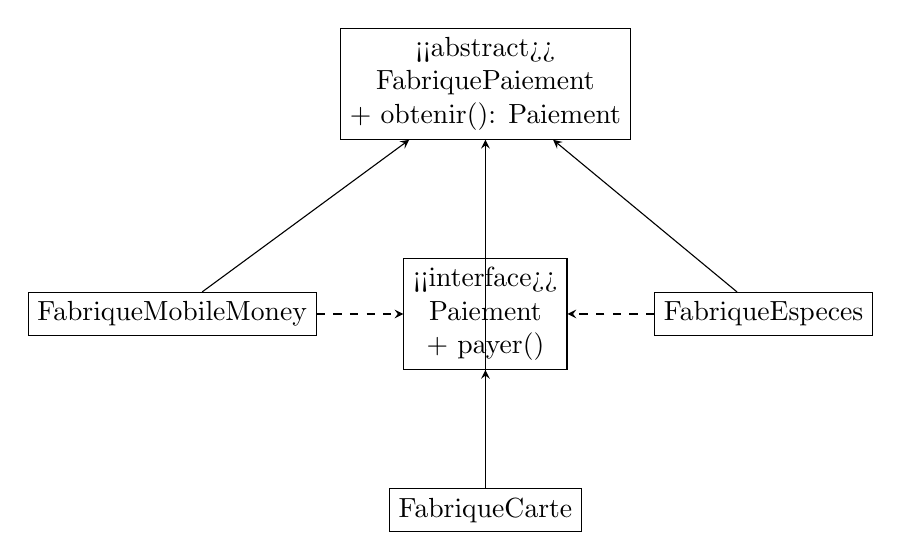
\begin{tikzpicture}[node distance=1.5cm and 1.1cm,>=stealth]
\node[draw,align=center] (f) {<<abstract>>\\FabriquePaiement\\+ obtenir(): Paiement};\node[draw,align=center,below=of f] (p) {<<interface>>\\Paiement\\+ payer()};
\node[draw,align=center,left=of p] (a) {FabriqueMobileMoney};\node[draw,align=center,below=of p] (b) {FabriqueCarte};\node[draw,align=center,right=of p] (c) {FabriqueEspeces};
\draw[->](a)--(f);\draw[->](b)--(f);\draw[->](c)--(f);\draw[->,dashed](a)--(p);\draw[->,dashed](b)--(p);\draw[->,dashed](c)--(p);
\end{tikzpicture}\end{center}
\subsection{Variante : quatre paiements}
On ajoute \texttt{VirementBancaire} et \texttt{FabriqueVirement}. Les fabriques existantes restent inchangées : c'est l'avantage du patron Factory.
\begin{lstlisting}
interface Paiement { String payer(); }
abstract class FabriquePaiement { Paiement obtenir(){ return creer(); } protected abstract Paiement creer(); }
class MobileMoney implements Paiement { public String payer(){ return "Mobile Money"; } }
class CarteBancaire implements Paiement { public String payer(){ return "Carte bancaire"; } }
class Especes implements Paiement { public String payer(){ return "Espèces"; } }
class VirementBancaire implements Paiement { public String payer(){ return "Virement bancaire"; } }
class FabriqueMobileMoney extends FabriquePaiement { protected Paiement creer(){ return new MobileMoney(); } }
class FabriqueCarte extends FabriquePaiement { protected Paiement creer(){ return new CarteBancaire(); } }
class FabriqueEspeces extends FabriquePaiement { protected Paiement creer(){ return new Especes(); } }
class FabriqueVirement extends FabriquePaiement { protected Paiement creer(){ return new VirementBancaire(); } }
\end{lstlisting}
\section{Analyse et dépôt GitHub}
Factory Method centralise la création dans une seule fabrique ; ajouter un nouveau type impose de modifier cette fabrique. Factory permet d'ajouter une nouvelle fabrique concrète sans modifier les classes existantes. Le dépôt GitHub public doit contenir les codes complets et les diagrammes Dia.
\end{document}
